\documentclass{article}
\usepackage{array}
\usepackage[affil-it]{authblk}
\usepackage[english]{babel}
% \usepackage{caption}
\usepackage{cite}
\usepackage{color}
\usepackage{courier}
\usepackage{graphicx}
\usepackage{hyperref}
\usepackage[utf8]{inputenc}
% \usepackage{listings}
% \usepackage{pgf-umlcd}
% \usepackage{pgf-umlsd}
\usepackage{multicol}
\usepackage{titling}
\usepackage{wrapfig}
\usepackage{xcolor}

\graphicspath{ {figures/} }


\setlength{\parindent}{0em}
\setlength{\parskip}{1em}
\definecolor{light-gray}{gray}{0.98}

% \lstset{
    basicstyle=\footnotesize\ttfamily, % Default font
    % numbers=left,              % Location of line numbers
    numberstyle=\tiny,          % Style of line numbers
    % stepnumber=2,              % Margin between line numbers
    numbersep=5pt,              % Margin between line numbers and text
    tabsize=2,                  % Size of tabs
    extendedchars=true,
    breaklines=true,            % Lines will be wrapped
    keywordstyle=\color{red},
    frame=b,
    % keywordstyle=[1]\textbf,
    % keywordstyle=[2]\textbf,
    % keywordstyle=[3]\textbf,
    % keywordstyle=[4]\textbf,
    commentstyle=\color{blue},
    stringstyle=\color{magenta}\ttfamily, % Color of strings
    showspaces=false,
    showtabs=false,
    xleftmargin=17pt,
    framexleftmargin=17pt,
    framexrightmargin=5pt,
    framexbottommargin=4pt,
    backgroundcolor=\color{light-gray},
    showstringspaces=false
}
\lstloadlanguages{ % Check documentation for further languages ...
     % [Visual]Basic,
     % Pascal,
     % C,
     % C++,
     % XML,
     % HTML,
     Java
}
% \DeclareCaptionFont{white}{\color{white}}
\DeclareCaptionFormat{listing}{\colorbox[cmyk]{0.43, 0.35, 0.35,0.01}{\parbox{\textwidth}{\hspace{15pt}#1#2#3}}}
\captionsetup[lstlisting]{format=listing,labelfont=white,textfont=white, singlelinecheck=false, margin=0pt, font={bf,footnotesize}}

\newcommand{\subtitle}[1]{%
  \posttitle{%
    \par\end{center}
    \begin{center}\large#1\end{center}
    \vskip0.5em}%
}
\newcommand{\uml}[2][1]{
	\begin{minipage}{.9\linewidth}
		\centering
		\resizebox{#1\linewidth}{!}{
			\input{uml/#2}
		}
	\end{minipage}
}


\begin{document}
\title{Technologies of Civic Participation}
\subtitle{Civic technologies and They Work for You}

\author{Candidate Exam Number: B136325}
\affil{Department of Informatics, University of Edinburgh, Scotland}

\date{Date: \today}

\renewcommand{\maketitlehookb}{\centering Version 0.1.5}

\maketitle

\begin{abstract}
\noindent An investigation of civic technologies focused upon They Work for You, and including descriptions of civic hacking and open data, along with taxonomies of civil tech. 
\end{abstract}

\pagebreak
\tableofcontents

\pagebreak
\addcontentsline{toc}{section}{List of figures}
\listoffigures

\pagebreak
\addcontentsline{toc}{section}{Introduction}
\section*{Introduction}
A civic technology is one that aids civic society, where civic society, in this conception, is considered to be the \emph{commons} mediating between commerce and government.
There are a broad range of civic technology (or \say{civic tech} for short) projects, both commercial and charitable, from social networks such as Facebook \cite{facebook} to election monitoring applications such as Ushahidi \cite{ushahidi}. 
From the perspective of the UK, arguably one of the most well known (and, indeed, one of the most established) civic tech projects is They Work for You, which provides automated, accessible data about government. 
An overview of They Work for You will be presented, along with a discussion of its aims and values. 
The challenges faced by the site will also be addressed, before it is compared with another project, Wikipedia \cite{wikipedia}, with regard to taxonomoies of civc tech.
Many civic tech projects, moreover, including They Work for You, encompasses elements from the open data movement,
and an overview of the movement will be presented directly below.


\addcontentsline{toc}{section}{Civic hacking}
\section*{Civic hacking}

  \addcontentsline{toc}{subsection}{Overview}
  \subsection*{Overview}
  It might be suggested that the stereotype of (not for profit) hackers is of an individual (usually a man) or a group (usually men) of programmers extracting information from (and, thereby, breaking into) a government or corporate computer system. In this gloss, hacking is akin to a high tech heist movie. Another way of understanding hacking might be to consider what it would appear to involve, namely , to hack iteratively at a large problem. And it is this conception of hacking that when applied to social problems gives rise to the term civic hacker. Thus the pre-existing outsider status of hackers is combined with commercial software engineering practices to address civil problems and to do so, for the most part, in a not for profit manner.


\addcontentsline{toc}{section}{Open data}
\section*{Open data}
  
    \addcontentsline{toc}{subsection}{Overview}
    \subsection*{Overview}
    One of the origins of the open data movement can be understood (at least from a sociological perspective) with regard to Anthony Gidden’s conception of trust. Giddens suggested that in modern or post-modern societies, and given the technological advances underlying the development of such societies, knowledge of the aspects of such societies becomes unknowable, producing an almost magical conception of trust. However, Gidden’s suggests that such trust is unstable and that it desires resolution, in terms of knowledge. It is suggested that such desire for understanding underlies at least some aspects of the modern open data movement.

From a historical perspective, however, the movement is often considered to have begun with the Freedom of Information Act (196*) signed into law in America by president LBJ. Although the act was arguably more limited than had been intended, it nevertheless provided a right to information (in this case about federal government).



\addcontentsline{toc}{section}{They Work for You}
\section*{They Work for You}
      
        \addcontentsline{toc}{subsection}{Overview}
        \subsection*{Overview}
        They Work for You is a civic technology that was founded by Tom Steinberg \cite{tom-steinberg} in 2003.
It provides information about political representatives, such as Members of Parliament (MPs) and Members of the Scottish Parliament (MSPs), across all four legislative assemblies in the UK.
The site is data driven.
That is, it provides an accessible user interface over data drawn, automatically, from secondary sources.
Originally, the data shown within the site was scraped (using a Wget \cite{wget} based script) from the website of Hansard \cite{hansard}, which is the official record of all UK parliamentary debates.
This led to a threat of legal action being taken against They Work for You by the government, because, at the time, no licence existed for the secondary use of Hansard data \cite{they-work-for-you-controversies}.
Whilst no prosecution took place, and whilst Tom Steinberg subsequently co-wrote a review for government called \emph{The Power of Information} \cite{power-of-information}, They Work for You
no longer scrapes data from the Hansard site, at all.
In fact, since the unveiling of the UK Government's Open Data Licence \cite{open-data-licence} (2010), They Work for You has drawn data directly from a government Application Programming Interface \cite{api} (or API).

        \addcontentsline{toc}{subsection}{Aims}
        \subsection*{Aims}
        Quoting directly from the They Work for You site, its aim is to \say{make it much easier for anyone to understand exactly what is going on in Parliament}.
It is suggested that that aim has been most fully realised with regard to the following three aspects of the site's implementation: (i) a front-end design that engenders accessibility; (ii) the curation of permanent URLs; and (iii)
the provision of open source and freely available code.
        
        \addcontentsline{toc}{subsection}{Implementation}
        \subsection*{Implementation}
        
        	\addcontentsline{toc}{subsubsection}{Accessible design: search box}
        	\subsubsection*{Accessible design: search box}
        	The screen shot within Figure \ref{fig:they-work-for-you-implementation-search-box} depicts the home page of the site,
and prominently displayed within the home page is a search box, which, amongt other types of entries, accepts postcode \cite{postcodes-uk} values.
When a user enters a postcode within the search box the site will subsequently display information about the MP associated with the entered post code.
This clear and simple process is a good example of how the design of the site engenders accessibility,
particularly for those users who do not know the name of their MP.

			\begin{wrapfigure}{r}{0.55\textwidth}
				\centering
				
\includegraphics[scale=0.20]{images/they-work-for-you-implementation-search-box}
				\caption{Search box}
				\label{fig:they-work-for-you-implementation-search-box}
			\end{wrapfigure}
        	
        	\addcontentsline{toc}{subsubsection}{Accessible design: text only}
        	\subsubsection*{Accessible design: text only}
        	A second way in which the design of the site engenders accessibility can be seen from the screen shot within Figure \ref{fig:they-work-for-you-implementation-text-only-lynx}.
The screen shot depicts a terminal (or console) based text only browser, and it is displaying the information from the They Work for You site for the current UK Labour Party leader Jermey Corbyn.
The text only browser displayed is called Lynx \cite{lynx}, which was created at the Univesity of Kanas in 1992, and which was successor to the first browser (known as 'WorldWideWeb' \cite{browser-history}) developed by Tim Bernes Lee \cite{tim-berners-lee}.

Relatively few modern web sites fully support text only browsing, due to the inclusion of client side JavaScript DOM manipulation.
However, text browsers are frequently the basis for text to speech browsing (or transformations) as used by those with disabilities, such as blindness.
As such, the fact that the site can be viewed via a text only browser is another demonstration of how its design engenders accessibility, and, hence, contributes to civil society.


			\begin{wrapfigure}{r}{0.55\textwidth}
				\centering
				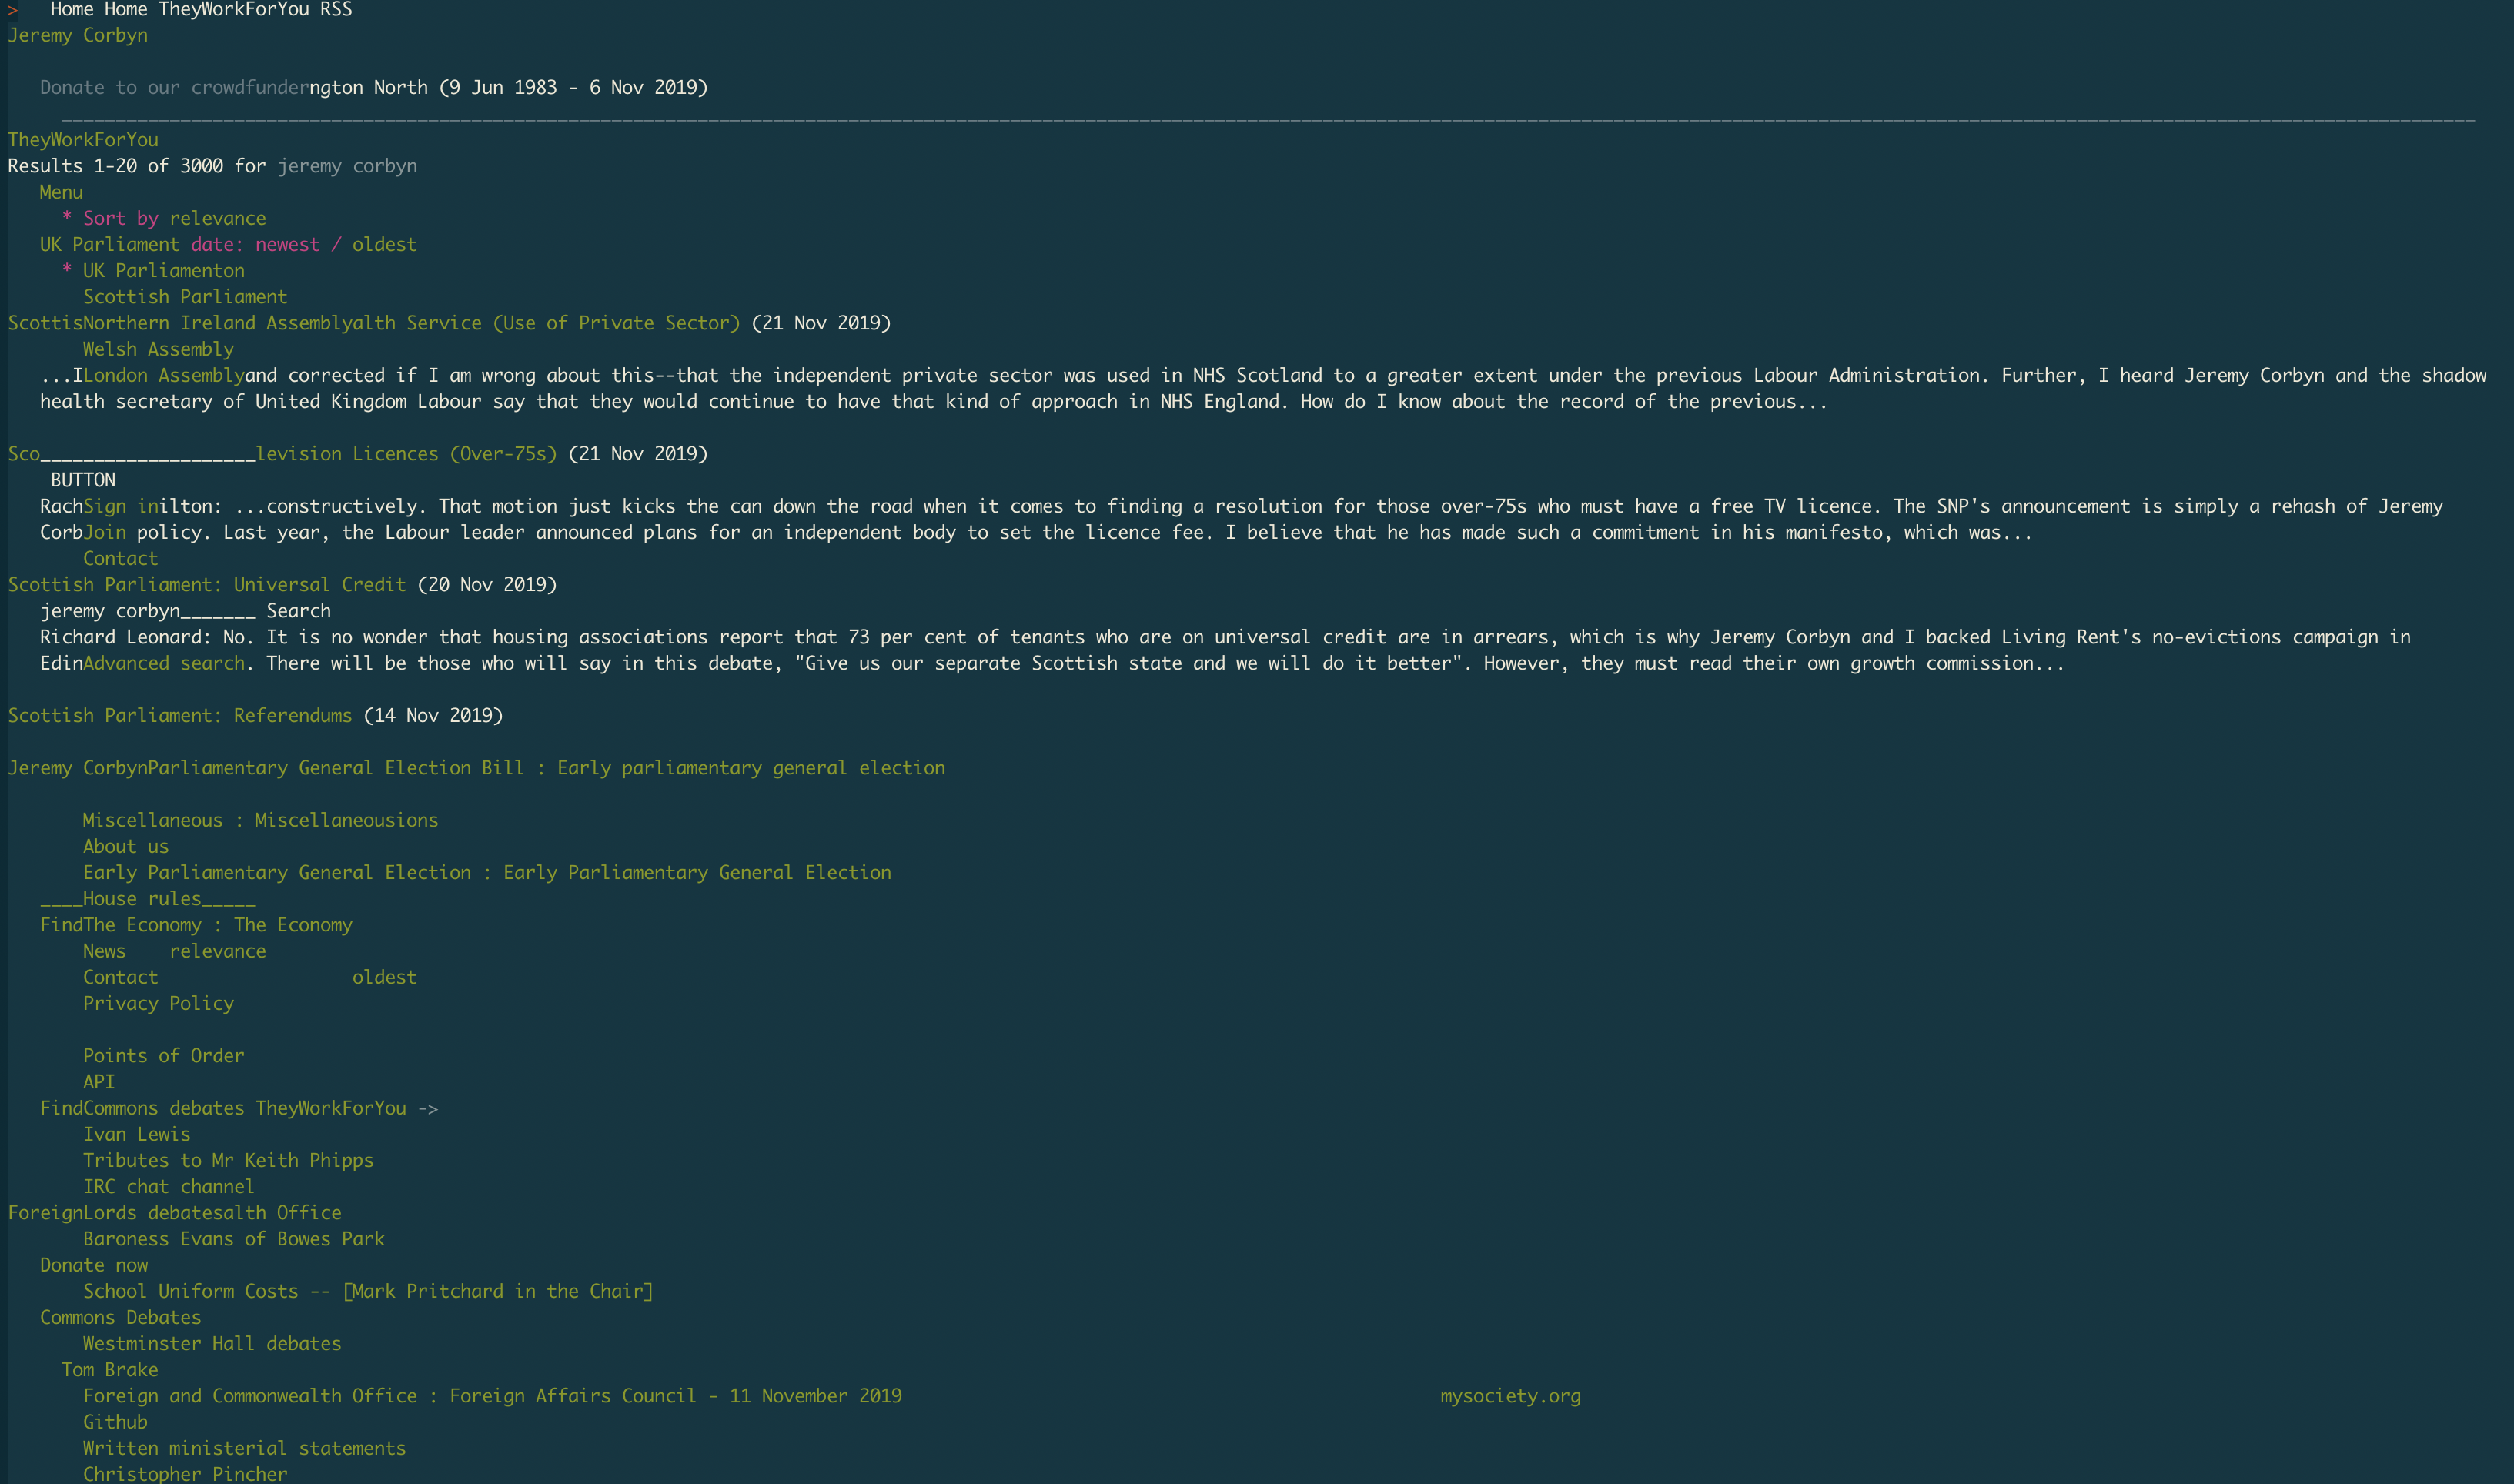
\includegraphics[scale=0.15]{images/they-work-for-you-implementation-text-only-lynx}
				\caption{They Work for You: text only browsing via Lynx}
				\label{fig:they-work-for-you-implementation-text-only-lynx}
			\end{wrapfigure}

        	\addcontentsline{toc}{subsubsection}{Permanent URLs}
        	\subsubsection*{Permanent URLs}
        	The second aspect of the implementation that enables the site to address its aims is the construction of permanent Uniform Resource Locators (URLs or web addresses).
The screenshot within Figure \ref{fig:/they-work-for-you-implementation-permanent-urls-1} shows a summary page (from within the They Work for You) for an exchange between two MPs in the House of Commons. 
The exchange, itself, is published by They Work for You with a permanent and unique URL.
In addition, each speech (or interjection) within the exchange can be viewed (and referenced) separately, as can be seen from the screenshot within Figure \ref{fig:they-work-for-you-implementation-permanent-urls-2}.
The construction of such URLs therefore provides a means of sharing (across the web) uniquely referenced debates and interjections. 
        	
			\begin{wrapfigure}{r}{0.55\textwidth}
				\centering
				
\includegraphics[scale=0.5]{images/they-work-for-you-implementation-permanent-urls-1}
				\caption{They Work for You: permanent page for a debate}
				\label{fig:/they-work-for-you-implementation-permanent-urls-1}
			\end{wrapfigure}

			\begin{wrapfigure}{r}{0.55\textwidth}
				\centering
				
\includegraphics[scale=0.3]{images/they-work-for-you-implementation-permanent-urls-2}
				\caption{They Work for You: permanent page for a single speech}
				\label{fig:they-work-for-you-implementation-permanent-urls-2}
			\end{wrapfigure}

			\begin{wrapfigure}{r}{0.55\textwidth}
				\centering
				
\includegraphics[scale=0.5]{images/they-work-for-you-implementation-permanent-urls-3}
				\caption{They Work for You: permanent URL for a single speech}
				\label{fig:they-work-for-you-implementation-permanent-urls-3}
			\end{wrapfigure}
					
         	\addcontentsline{toc}{subsubsection}{Open source}
        	\subsubsection*{Open source}
        	The third aspect of the site that enables it to contribute to civicl society 
provision of open source code freely available 

This has been packaged by MySociety is a tool called Pombola
And the screenshot depicts info about Pombola showing that it is currently being used in South Africa and Kenya

			\begin{wrapfigure}{r}{0.55\textwidth}
				\centering
				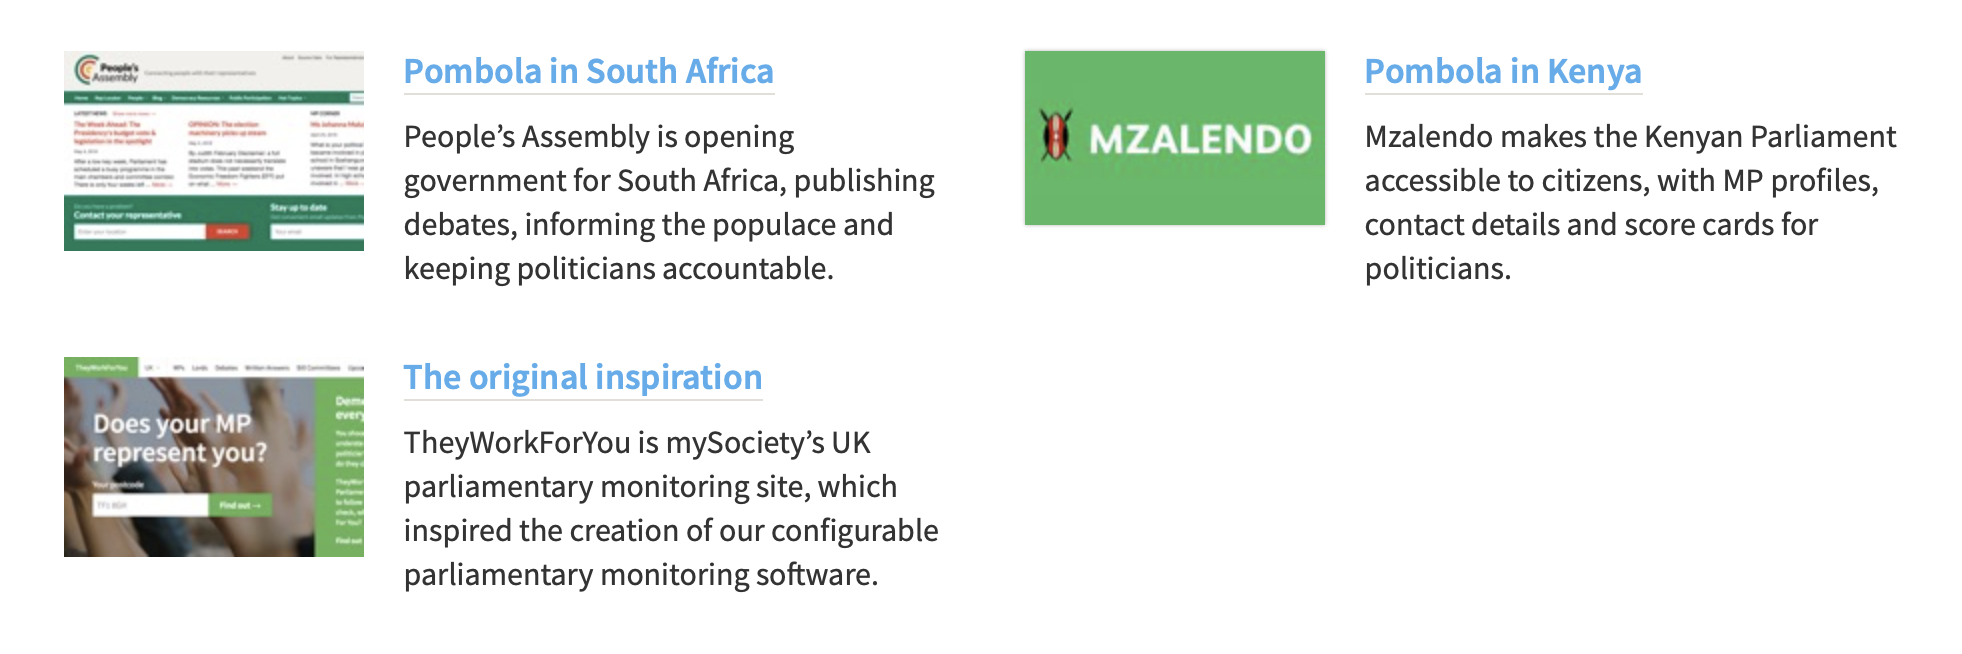
\includegraphics[scale=0.4]{images/they-work-for-you-implementation-open-source-pombola}
				\caption{They Work for You: Pombola}
				\label{fig:they-work-for-you-implementation-open-source-pombola}
			\end{wrapfigure}
			
			\begin{wrapfigure}{r}{0.55\textwidth}
				\centering
				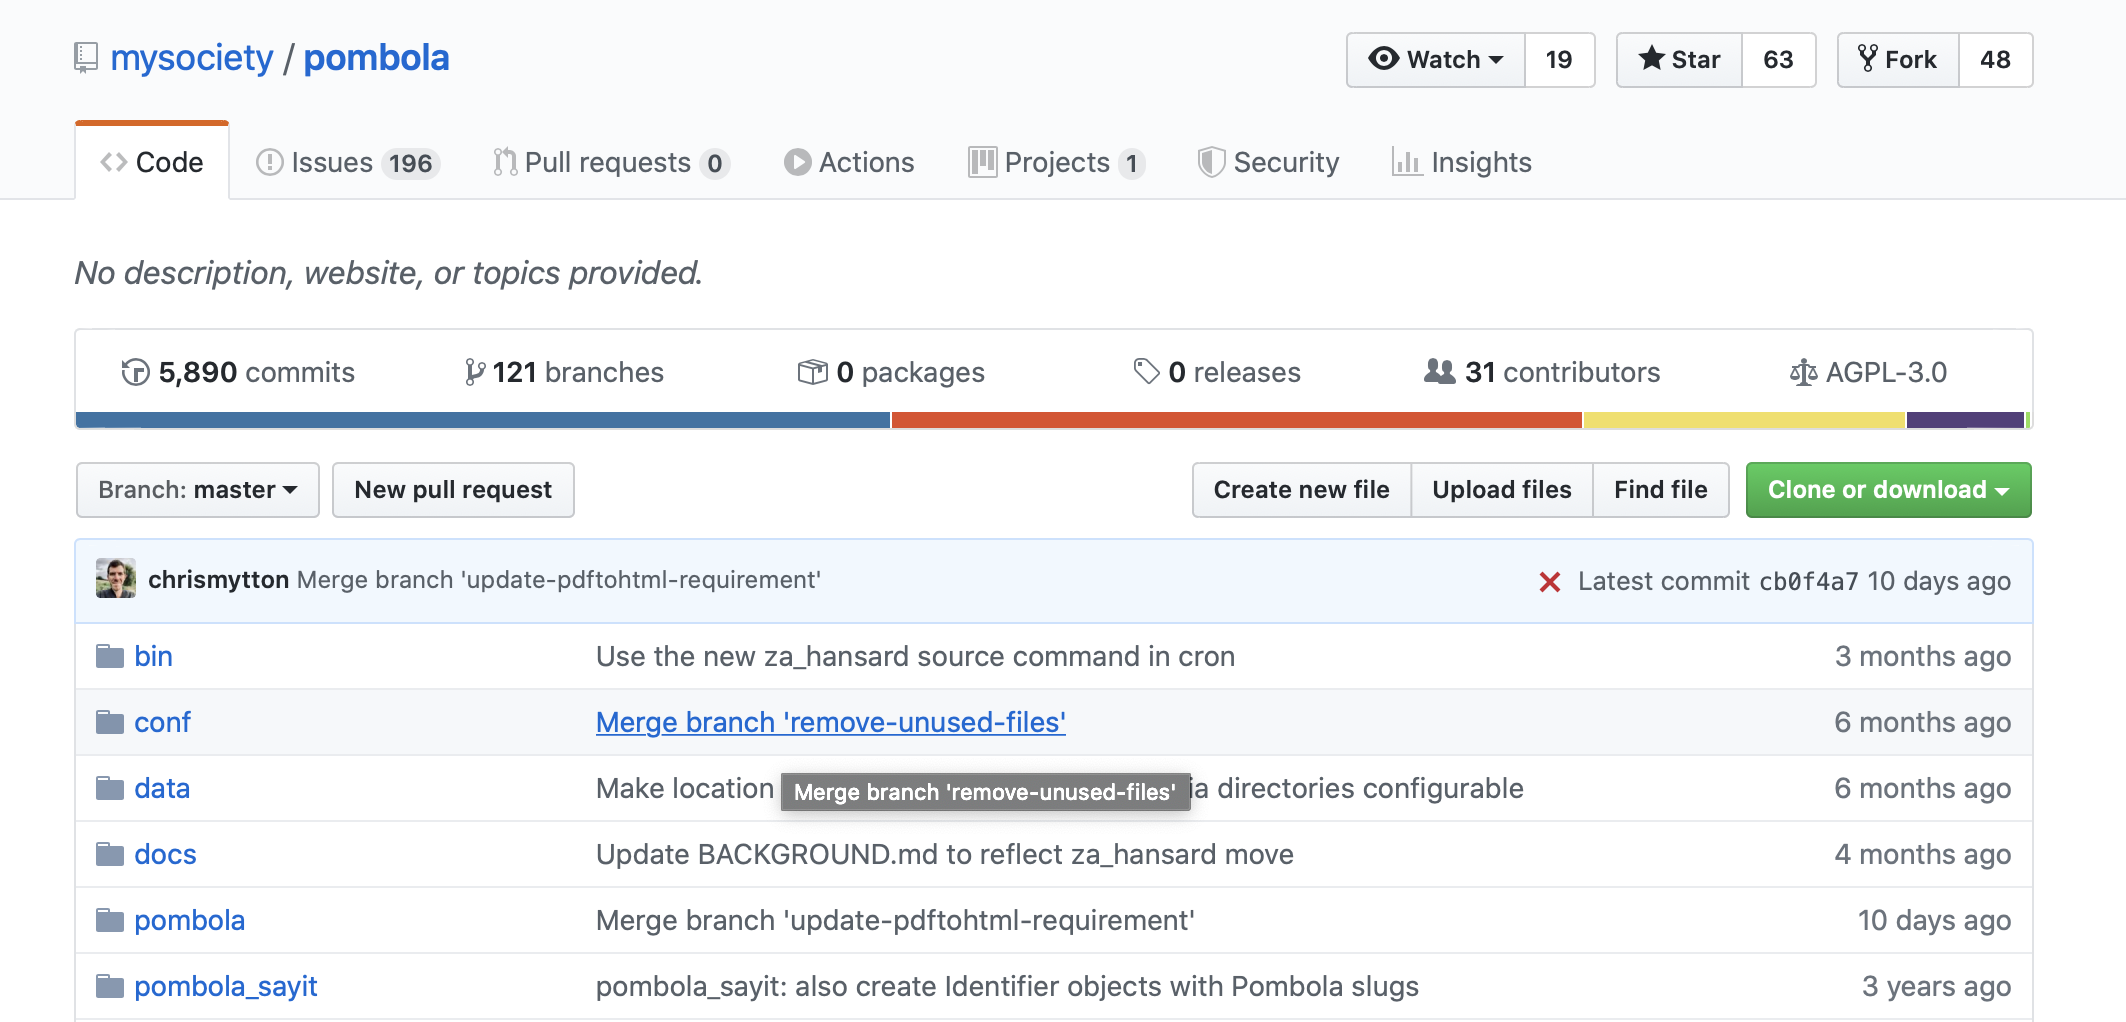
\includegraphics[scale=0.4]{images/they-work-for-you-implementation-open-source-github}
				\caption{They Work for You: GitHub}
				\label{fig:they-work-for-you-implementation-open-source-github}
			\end{wrapfigure}
						
         	\addcontentsline{toc}{subsubsection}{Summary}
        	\subsubsection*{Summary}
        	Taken toegther, They Work for You contributes to civil society through its implementation, whose key aspects are: (i) accessible design; (ii) the construction of permanent URLs; and (iii) open source and freely available code, which, additionally (and through Pombola) aids the development of civil society in secondary countries.

        	        	          	  
        \addcontentsline{toc}{subsection}{Values}
        \subsection*{Values}

         	\addcontentsline{toc}{subsubsection}{Overview}
        	\subsubsection*{Overview}
        	It is suggested that the values inscribed within They Work for You are the civic virtues of cooperation and data sharing.
On the one hand, the site enables data about parliament to be more accessible, as exemplied by the design of the search box and the ability of the site to be viewed via text only browser, such as Lynx. 
On the other, the code has been packaged and is freely available, with a open source XXX license. 

         	\addcontentsline{toc}{subsubsection}{Strengthen civil society}
        	\subsubsection*{Strengthen civil society}
        	MOVING ON NOW TO SLIDE 12 TO ADDRESS THE VALUES INSCRIBED IN THE TECHNOLOGY 
I WOULD SUGGEST - PRIMARY VALUES ARE Cooperation and sharing of data
  HOWEVER, THE SAME TECHNOLOGIES THAT enABLe THOSE POSITIVE VALUES
MAY GIVE RISE TO CONCERNS data driven nature of the site 
WHICH IT IS SUGGESTED MAY LEAD TO a focus on MPs voting patterns
      and not the broader aspects of their roles within a community - or in indeed in government.

         	\addcontentsline{toc}{subsubsection}{Data object}
        	\subsubsection*{Data object}
        	Appendix 4 - Ian Murray

			\begin{wrapfigure}{r}{0.55\textwidth}
				\centering
				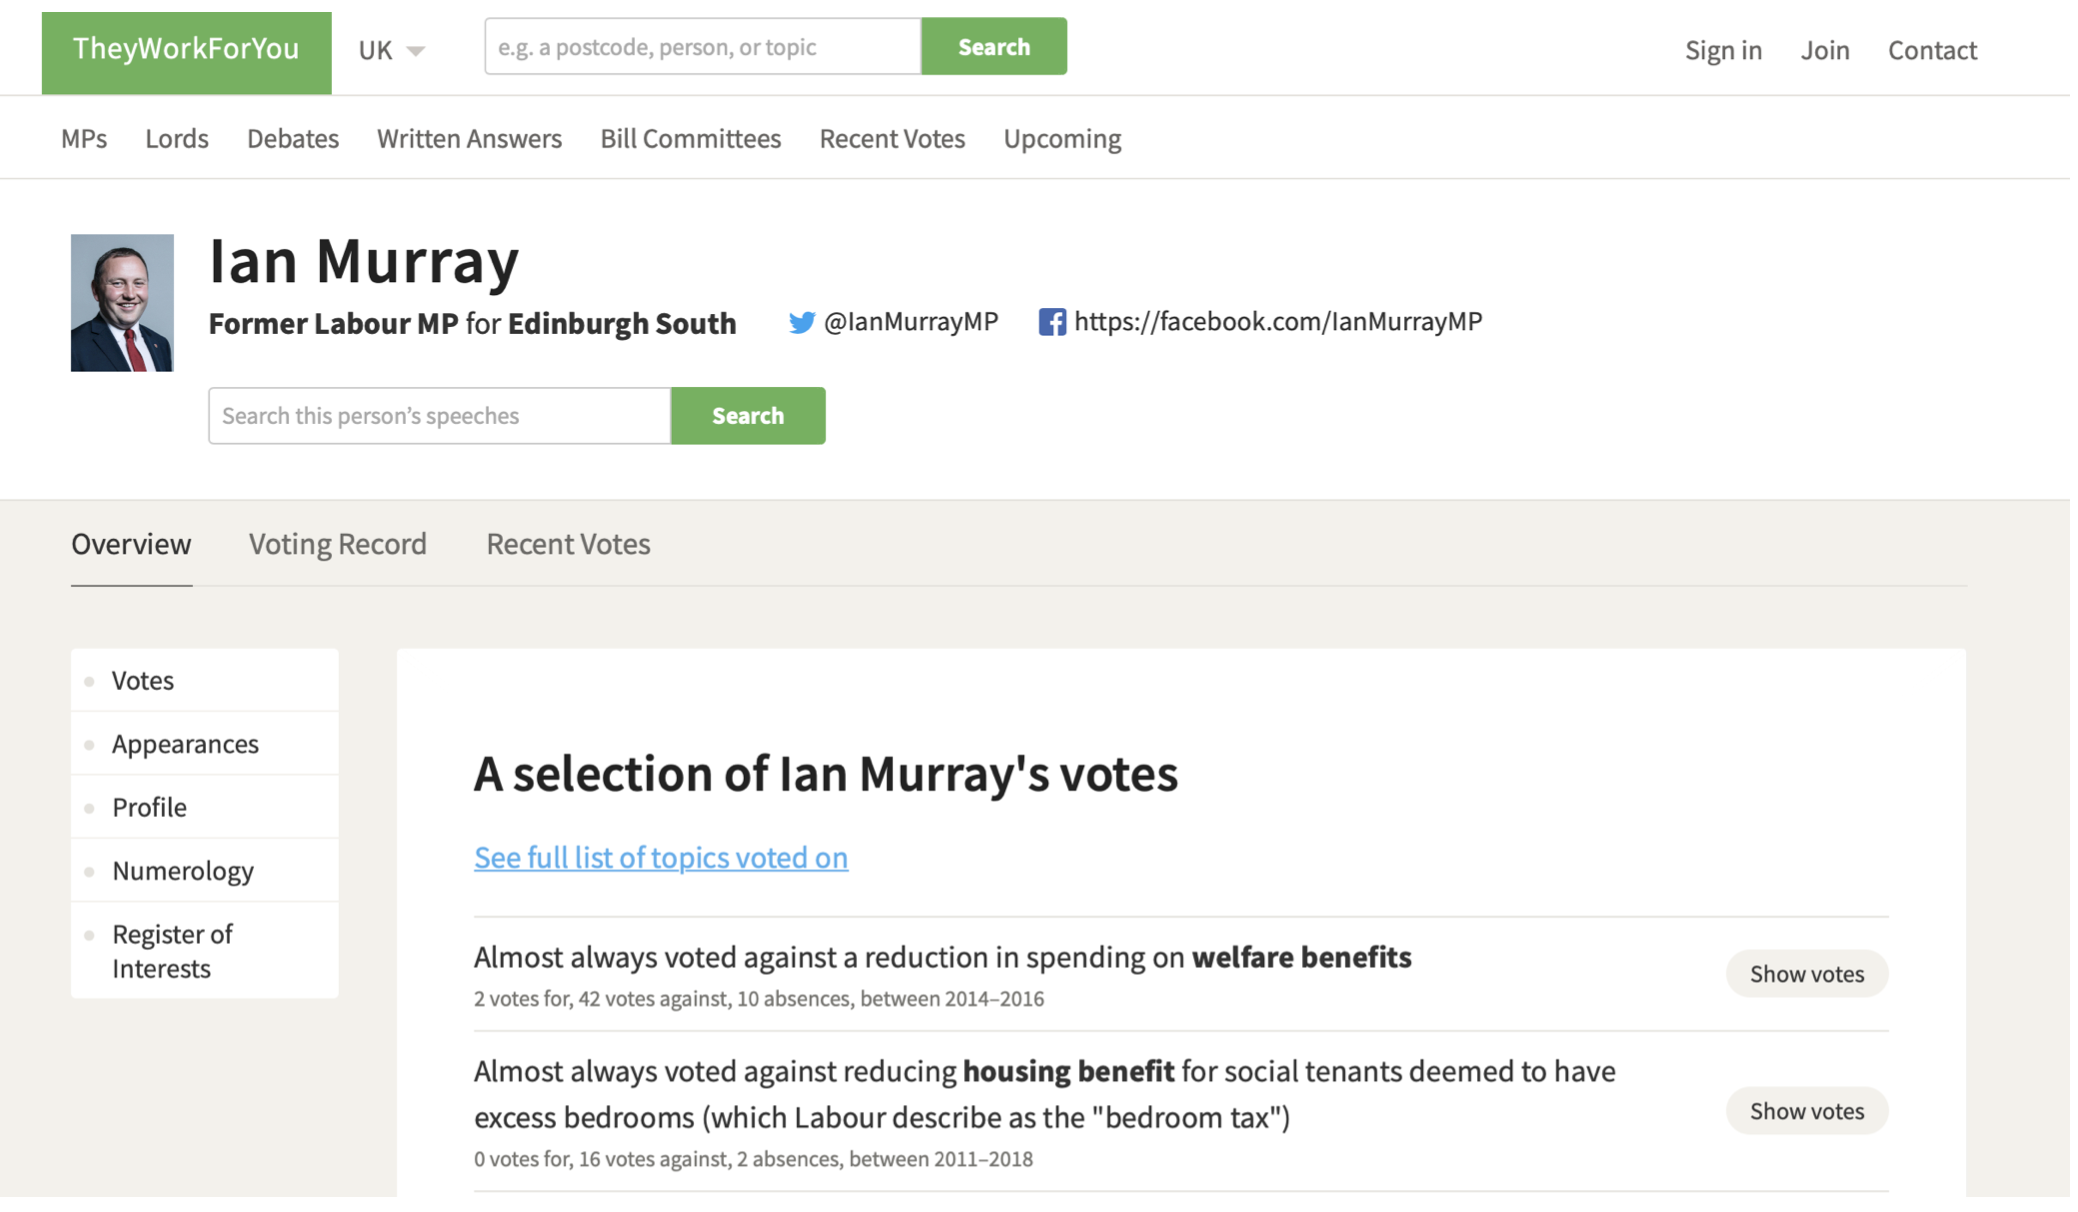
\includegraphics[scale=0.5]{images/they-work-for-you-ian-murray}
				\caption{They Work for You: generated page for MP Ian Murray}
				\label{fig:they-work-for-you-ian-murray}
			\end{wrapfigure}
			
         	\addcontentsline{toc}{subsubsection}{Data object: response}
        	\subsubsection*{Data object: response}
        	\begin{figure}[h]
  \centering
  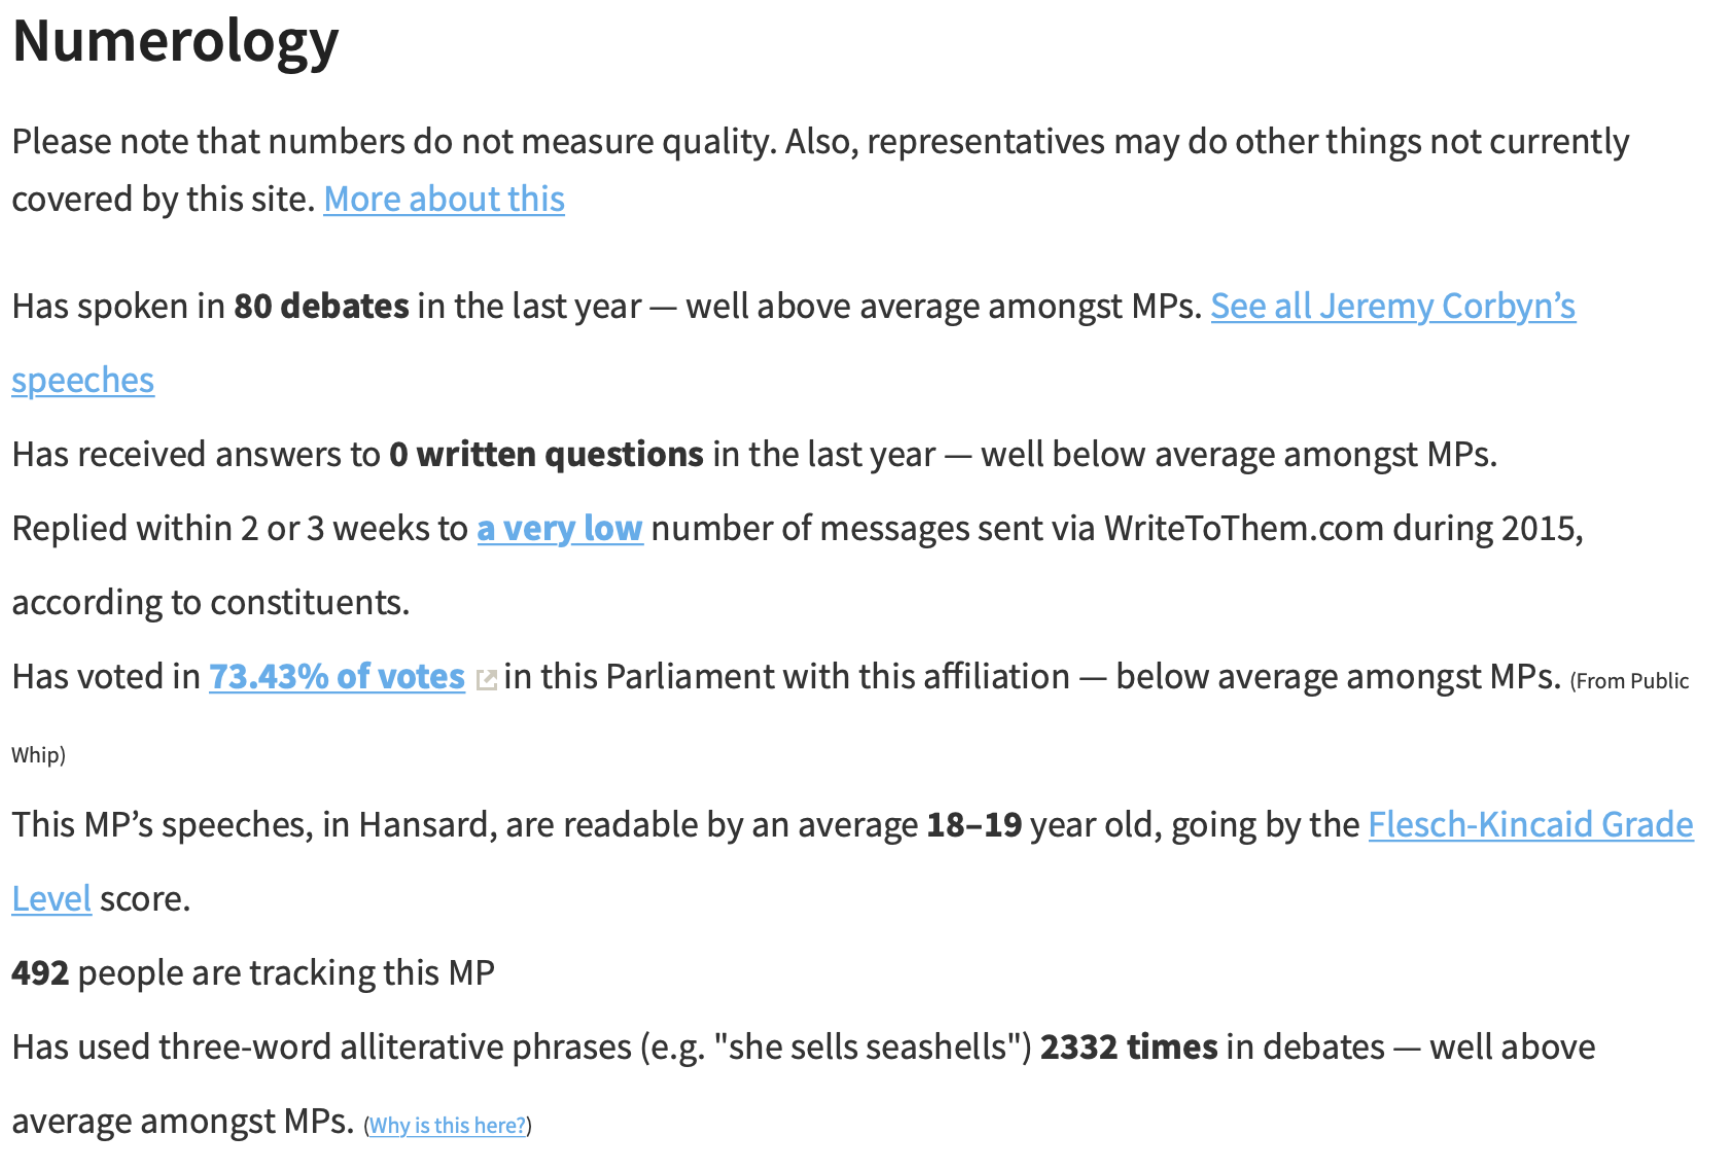
\includegraphics[scale=0.3]{images/they-work-for-you-numerology}
  \caption{They Work for You: numerology section}
  \label{fig:they-work-for-you-numerology}
\end{figure}

That being said, They Work for You are aware of the problem.
Within the page associated with each MP, they have added a section called Numerology, 
as can be seen from the screen shot within Figure \ref{fig:they-work-for-you-numerology},
which highlights some of the problem around a data driven and potentially data object perspective.

			\begin{wrapfigure}{r}{0.55\textwidth}
				\centering
				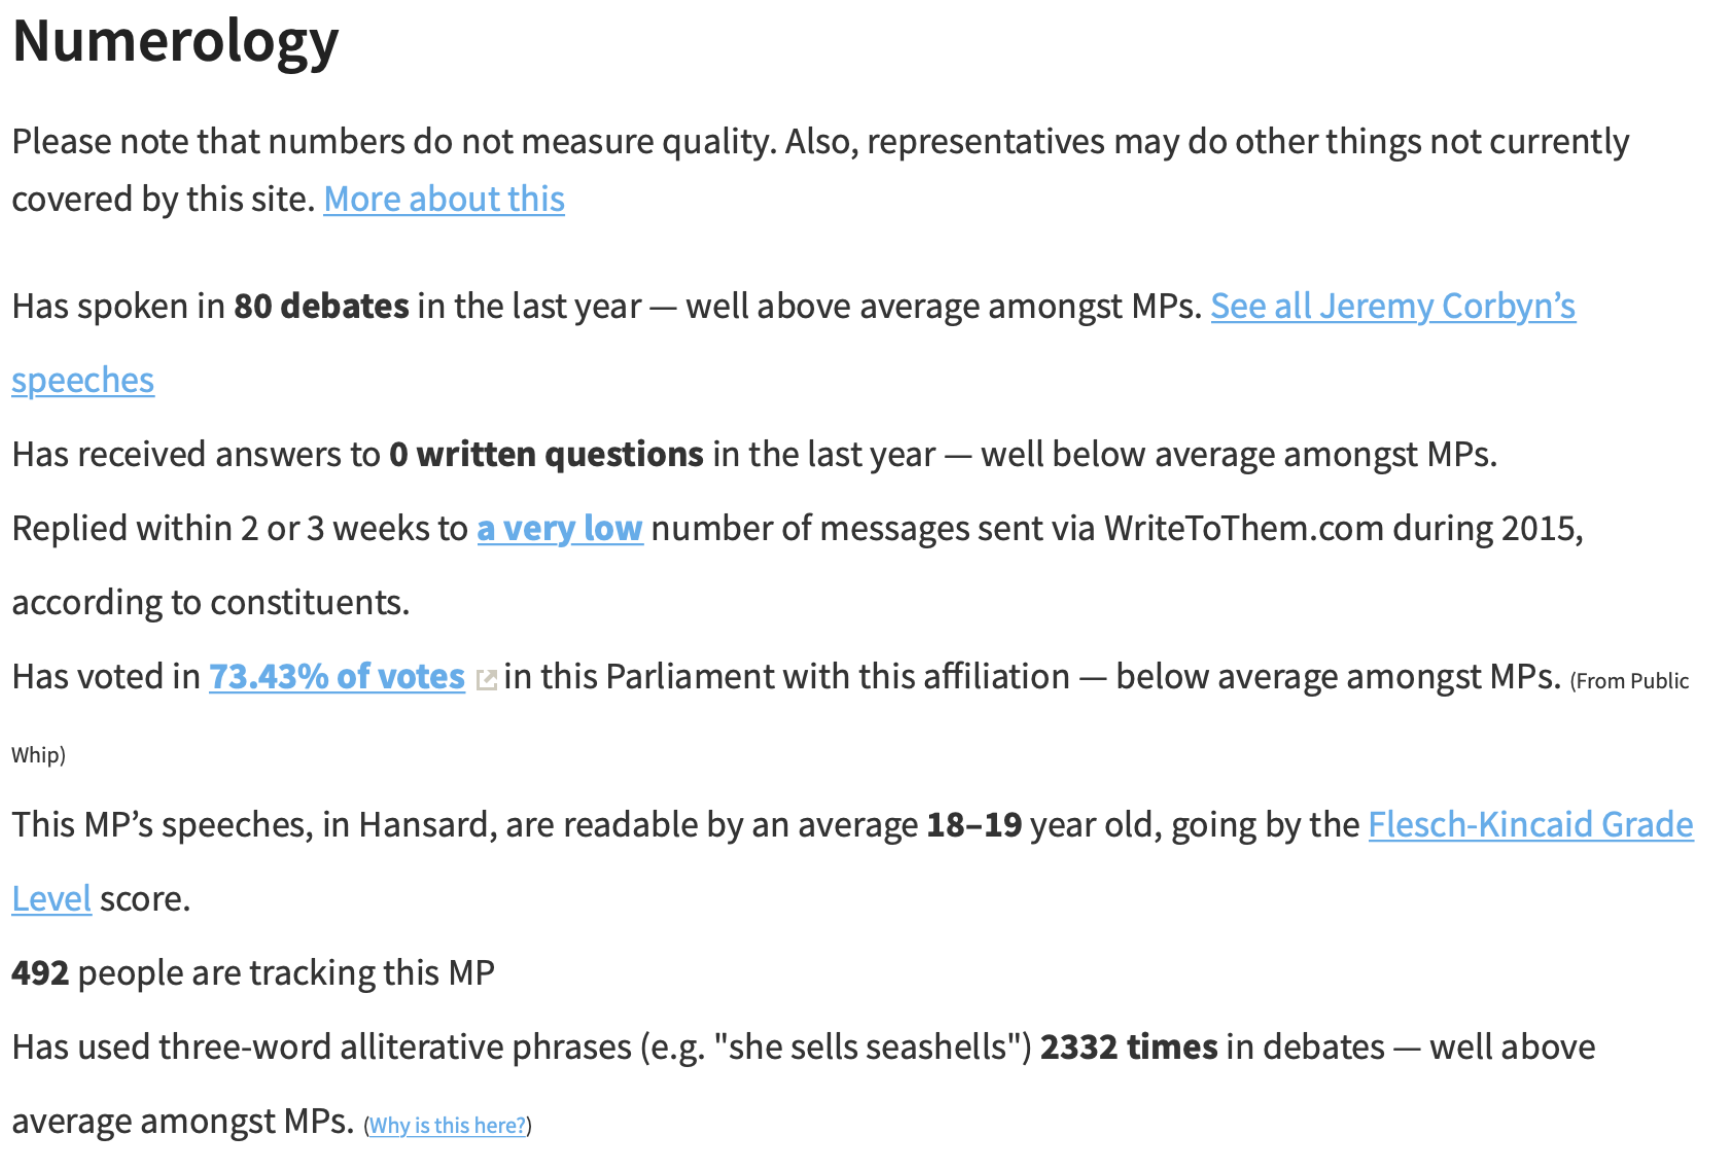
\includegraphics[scale=0.5]{images/they-work-for-you-numerology}
				\caption{They Work for You: numerology section}
				\label{fig:they-work-for-you-numerology}
			\end{wrapfigure}

         	\addcontentsline{toc}{subsubsection}{Summary}
        	\subsubsection*{Summary}
        	

        	        	        	        	        	                	        	          	     	
        \addcontentsline{toc}{subsection}{Challenges}
        \subsection*{Challenges}
        
        	\addcontentsline{toc}{subsubsection}{Users}
        	\subsubsection*{Users}
        	One of the primary challenge faced by They Work for You in fulfilling such contributions to civil society concerns the type of users accessing the site.
Although They Work for You do not publish user statistics, the site has an Alexa rank of approximately 125,000 \cite{alexa-rank}, suggesting, at least aneecdotally, that the site receives around 20,000 user visits per month.
Whilst the contributors to the development of the site should be proud of such user enagagement, it is suggested, however, that there may be an element of self selection amongst those using the site; that is, they are already interested in politics.
Moreover, such self selection may ameliorate the strength of the contribution of the site as a whole to the general public and, thereby, civil society.    

        	\addcontentsline{toc}{subsubsection}{Web analytics}
        	\subsubsection*{Web analytics}
        	Figure \ref{fig:they-work-for-you-challenges-google-analytics} depicts a screen shot of network traffic generated by the They Work for You site when viewed using the Chrome browser.
The five entries towards the bottom of the screenshot show that the site is sending information about user activity to Google Analytics \cite{google-analytics} on an approximately second by second basis.
That is, the client browser that that the author of this essay used to view the site is sending information to Google Analytics.
This finding suggests that They Work For You as an organisation do have access to statistics about user activity on their site.
However, given that They Work for You is a small charitable organisation, it may well be the case that make use of the free version of Google Analytics.
If that is the case, then the rights to the aggregated analytics data are held by Google, and that may explain why they don’t publish data about usage of the site.
        	
			\begin{wrapfigure}{r}{0.55\textwidth}
				\centering
				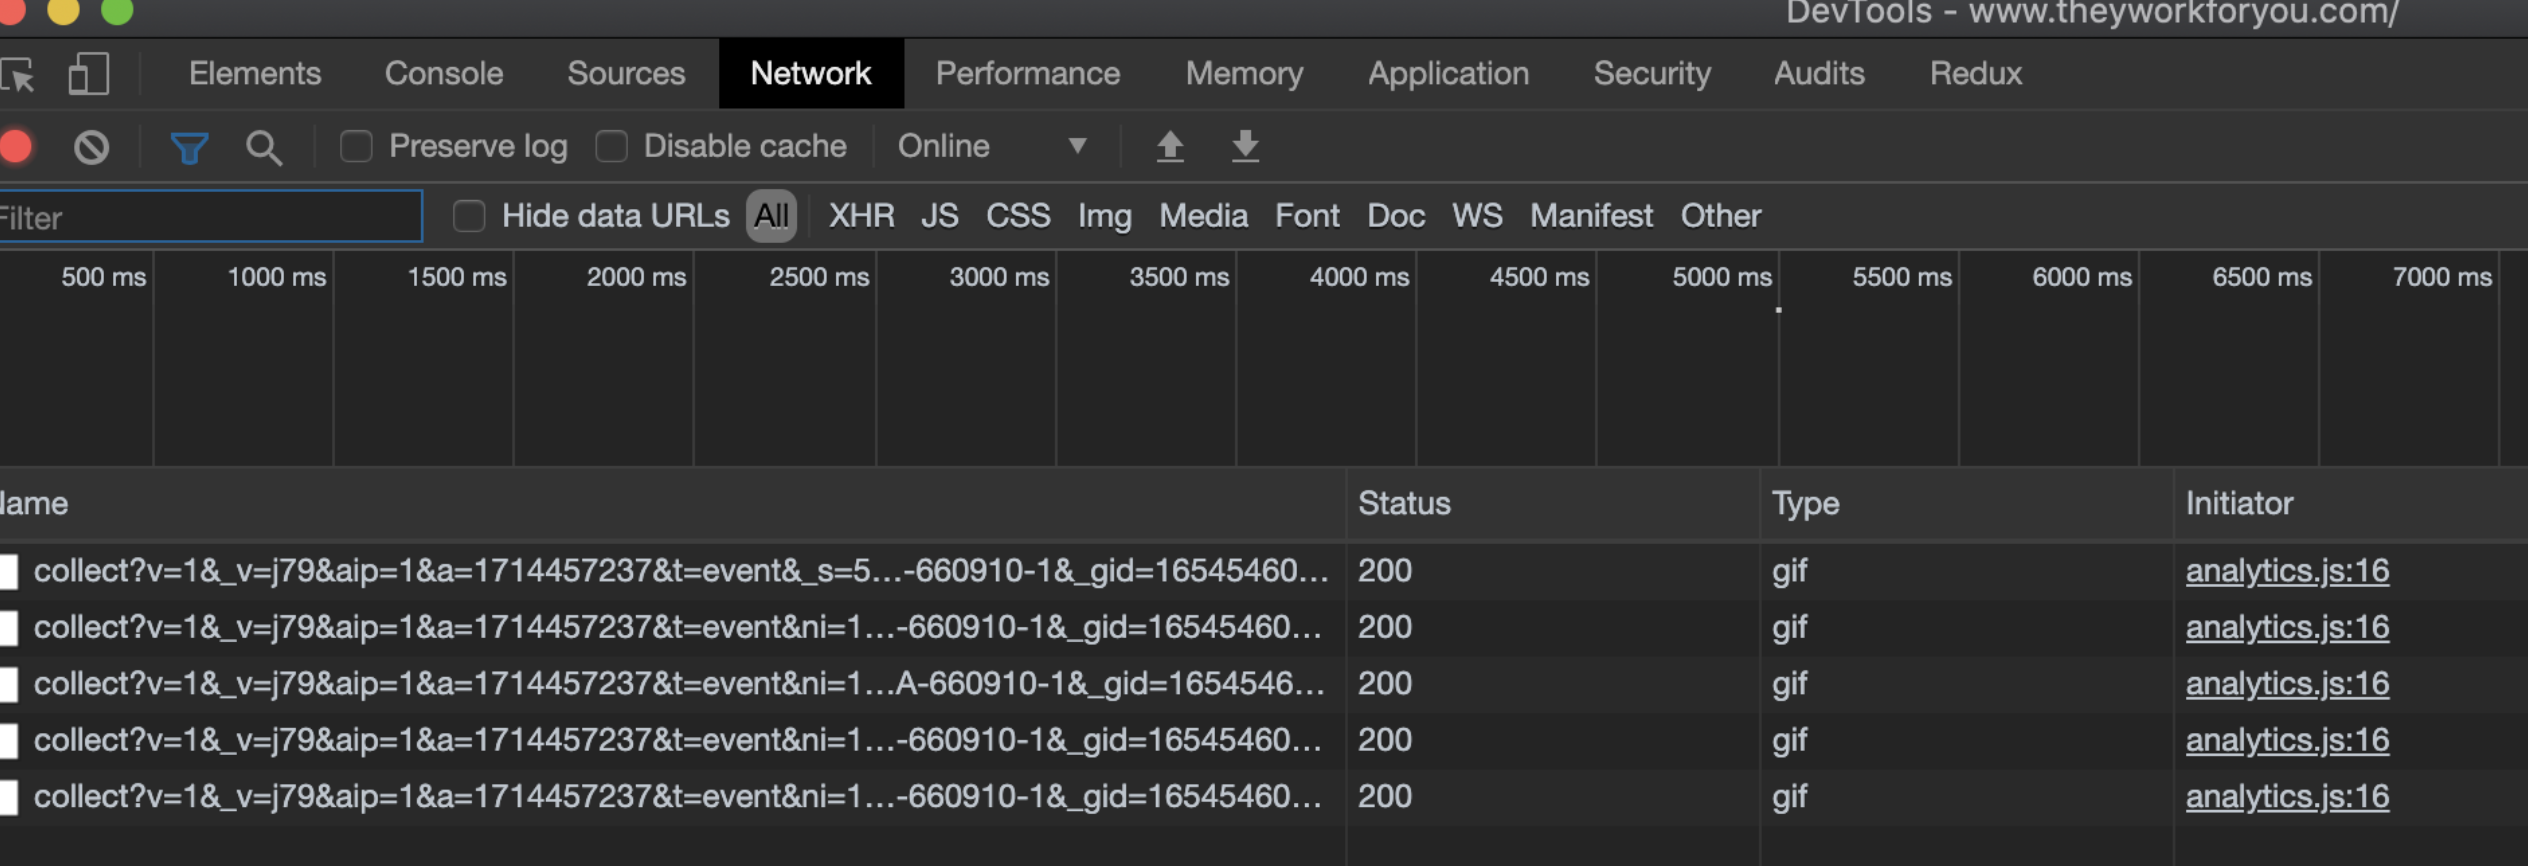
\includegraphics[scale=0.4]{images/they-work-for-you-challenges-google-analytics}
				\caption{They Work for You: Google analytics}
				\label{fig:they-work-for-you-challenges-google-analytics}
			\end{wrapfigure}
			
        	\addcontentsline{toc}{subsubsection}{Finance}
        	\subsubsection*{Finance}
        	That being said, and according to a Guardian article in 2008
	The Work For You via My Society undertook paid work for the government to produce the UK e-petition site,
		A SCREENSHOT OF WHICH CAN BE FOUND IN SLIDE 11.
	In addition, the They Work For You ofer a paid for API - Application Programming Interface    

			\begin{wrapfigure}{r}{0.55\textwidth}
				
\includegraphics[scale=0.4]{images/they-work-for-you-challenges-finance}
				\caption{They Work for You: banner advert for donations}
				\label{fig:they-work-for-you-challenges-finance}
			\end{wrapfigure}
			
			\begin{wrapfigure}{r}{0.55\textwidth}
				\centering
				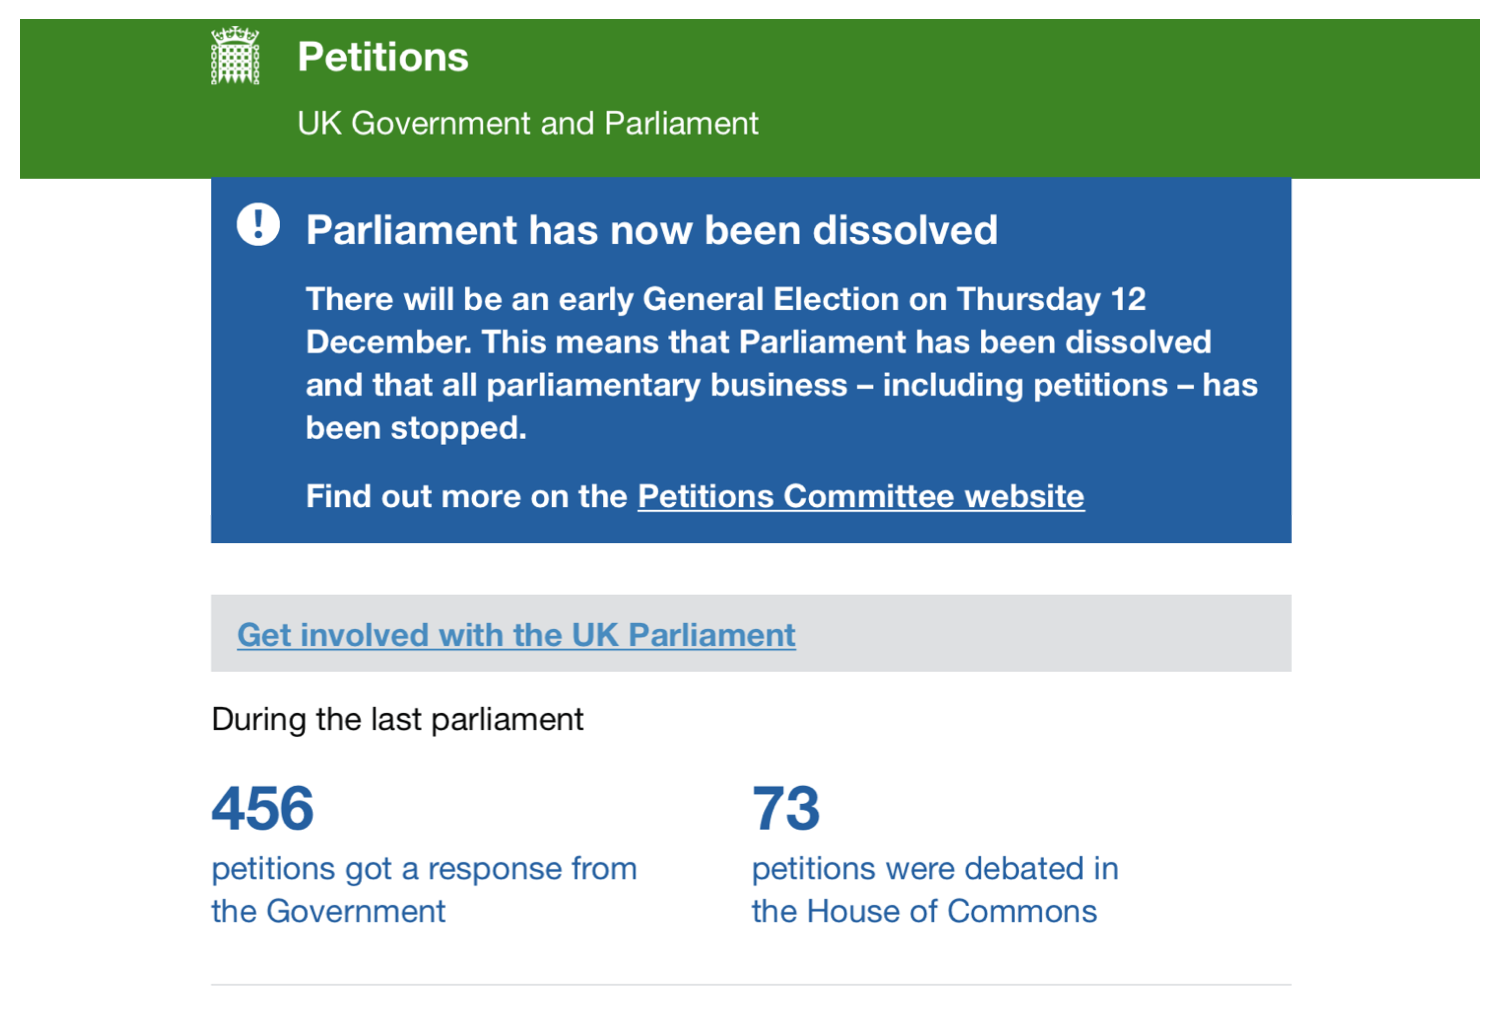
\includegraphics[scale=0.4]{images/e-petition-site}
				\caption{UK Government: E-Petition web site}
				\label{fig:e-petition-site}
			\end{wrapfigure}
						
        	\addcontentsline{toc}{subsubsection}{Summary}
        	\subsubsection*{Summary}
        	In short, two of the challenges faced by They Work for You in fullfilling its aims towards civic society are: (i) how to promote an understanding of politics beyond those already interested in the subject, which is an issue that can be further addressed via web analytics; and (ii) they may face financial pressures, though as mentioned the overall picture of their finances may be more complex than it at first seems.
        	
        	 
\addcontentsline{toc}{section}{Taxonomies of civic technology}
\section*{Taxonomies of civic technology}

        \addcontentsline{toc}{subsection}{Overview}
        \subsection*{Overview}
        In XXX Micah Sifry presented a visual depiction of a cartesian taxonomy of civic tech, as shown within Figure {fig:taxonomy-sifry}.
The vertical axis of the taxonomy represented a scale of participatory engagement from thin to click,
with 'thin' representing simply clicking a like button,
and 'thick' representing activities more involved.
The horizontal axis of the taxonomy depcits a scale of the aggregated outcome of such engagement, 
from purely symbolic to those that promote lasting impactful change.
        
			\begin{wrapfigure}{r}{0.55\textwidth}
				\centering
				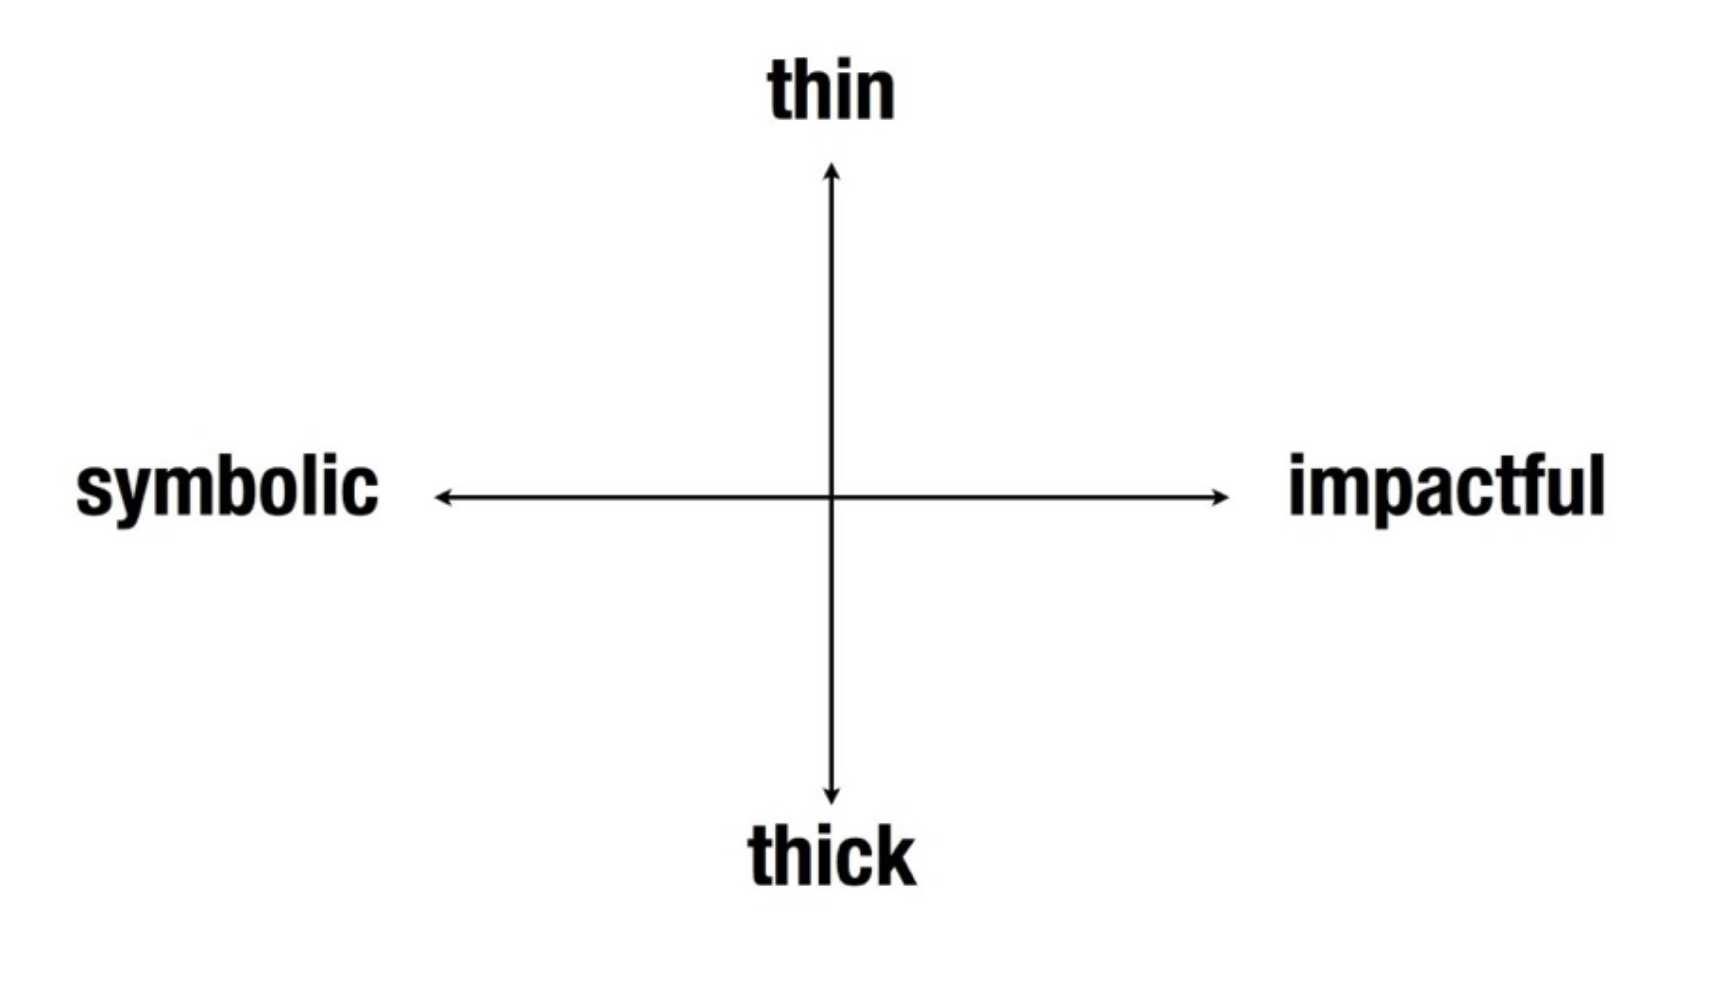
\includegraphics[scale=0.5]{images/taxonomy-sifry}
				\caption{Taxonomies of civic technology: Sifry}
				\label{fig:taxonomy-sifry}
			\end{wrapfigure}
			        
         \addcontentsline{toc}{subsection}{Groups}
        \subsection*{Groups}
        Micah Sifry’s taxonomy offers a powerful means of \emph{discriminating} between and identifying different types of civic technologies.
However, it is suggested that it does not offer a comprehensive means of \emph{describing} individual projects.
For instance, the taxonomy does not (directly) incorporate the nuanced conception of group membership outlined by Noveck \cite{noveck}.

In addition, it is also worth noting that civic technologies may give rise to \emph{secondary} groups, which blur the distinction between end users and volunteers.
Earlier iterations of the They Work for You site contained a ranking of MPs by (in one case) the number of written questions that the MPs has submitted to ministers.
As the site become more well known, anecdotal evidence suggested that a small number of MPs had attempting to \emph{game} the system by asking their advisors to make additional written requests (using the MPs name), and, thereby, improve their ranking on the site.
This is an interesting circular example, where (if true) the behaviour of MPs was modified by the presence of the ranking indicator within the site.
They Work for You have since removed such rankings.
        
         \addcontentsline{toc}{subsection}{Infrastructure}
        \subsection*{Infrastructure}
        A second issue not directly addressed by Micah Sifry’s taxonomy concerns the technologies underlying a civic tech project.
This issue is of particular importance when such projects are undertaken in regions of the world without freely accessible web networks.
In addition, and with particular regard to the open data movement in the UK, much of the UK government's open data is hosted using Microsoft Azure cloud based systems.

\addcontentsline{toc}{section}{Pipeline taxonomy}
\section*{Pipeline taxonomy}

        \addcontentsline{toc}{subsection}{Overview}
        \subsection*{Overview}
        PIPELINE TAXONOMY of civic tech
	Low Level technologies - such as servers - AND OR accessibility of open web networks - important when considering civic tech in countries with restrictive web practicies
	MovING FORWARD TO THE RIGHT the taxonomy addresses the design of individual civic tech projects
	IT then encompasses the types of engagement such projects offer - group membership
  Lastly, it  finishes with a phrase coined by Tom Steinberg (the founded of My Society) NAMELY - civic power. That is, what types of civic power does a project engender.
  
	I would suggest that this pipeline taxonomy offer strong descriptive power (per individual civic tech project) but, unfortunately, lacks the discriminative clarity of the taxonomy proposed by Micah Sifry.

			\begin{wrapfigure}{r}{0.55\textwidth}
				\centering
				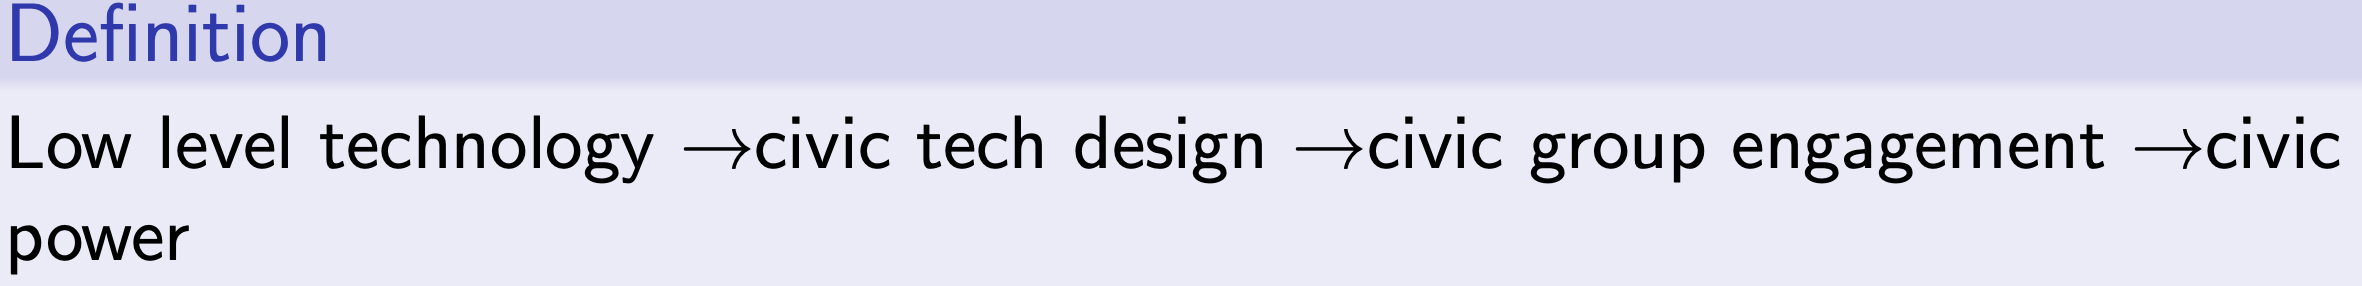
\includegraphics[scale=0.5]{images/taxonomy-pipeline}
				\caption{Pipeline taxonomy}
				\label{fig:taxonomy-pipeline}
			\end{wrapfigure}

        \addcontentsline{toc}{subsection}{Wikipedia}
        \subsection*{Wikipedia}
        The \emph{pipeline} taxonomy will be used to compare They Work for You with another civic technology, Wikipedia.
Wikipedia was co-founded by Jimmy Wales \cite{jimmy-wales} and Larry Sanger \cite{larry-sanger} in 2001 and has grown since then to become one of the world's largest user maintained repositories of knowledge, with approximately 30 million registered volunteers (or \emph{Wikipedians}) writing and maintaining articles.

From a low level perspective, both They Work for You and Wikipedia are (or were) written in the open source PHP scripting language \cite{php}.
In terms of design and content, Wikipedia (as mentioned) is user maintained by a large group of volunteers.
In contrast, the content within They Work for You is automatically generated from API data feeds.
Moreover, the code handling and displaying the data represented by such feeds would appear to be maintained by a relatively small team of volunteers.
Consequently, it is suggested that the different forms of content generation give rise to differing volunteer groups. Wikipedia volunteers may have a sense of ownerships or involvement with a relatively small part of the overall encyclopedia.  That being said, they are directly concerned with what is displayed on the web. In contrast, the volunteers working for They Work for You may be considered to operate in a more detached manner. 
Lastly, whilst both They Work for You and Wikipedia promote the civic power of open knowledge, Wikipedia does so (directly) by enabling end users to become volunteers. 

        \addcontentsline{toc}{subsection}{Further research}
        \subsection*{Further research}
        Richard Rogers
                
        \addcontentsline{toc}{subsection}{Summary}
        \subsection*{Summary}
        I would suggest that this pipeline taxonomy offer strong descriptive power (per individual civic tech project) but, unfortunately, lacks the discriminative clarity of the taxonomy proposed by Micah Sifry.
               
\addcontentsline{toc}{section}{Conclusion}              
\section*{Conclusion}
\input{sections/conclusion.tex}

\pagebreak
\addcontentsline{toc}{section}{Appendix}              
\section*{Appendix}

\pagebreak
\addcontentsline{toc}{section}{References}              
\bibliography{references} 
\bibliographystyle{ieeetr}

\end{document}